\clearpage
\section{Hardware}

\subsection{Raspberry PI}
The Raspberry PI is a small computer in the form of a single board with a system on a chip. The SoC is a BCM2835 licensed from Broadcom. It has an ARM11v6 CPU running at 700 MHz with 256 (model A) or 512 MB (model B) SDRAM shared with the on board GPU.
\begin{figure}[h]
    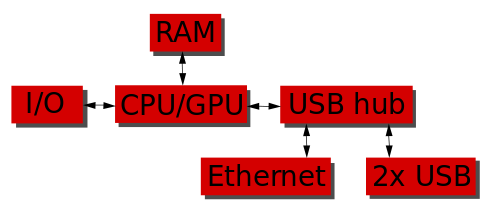
\includegraphics[width=0.5\textwidth]{hardware/raspberrypi_block_function}
    \caption{Layout of the functional blocks on the PI}
    \label{fig:pi_blockdiagram}
\end{figure}

\subsection{Configuration}
The PI comes with a number of different options for configuration. It can be overclocked and the amount of memory split with the shared memory GPU can be set at boot using {\tt /boot/config.txt}.
Most unofficial documentation states that it requires a minimum of 16MB of RAM, but we were unable to get the PI to boot with less than 48 MB. With less than 48, it seems the system never gets to boot.
The setting on our running hardware is therefore {\tt gpu\_mem\_512=48}.

The Raspberry also allows for easy overclocking without voiding the warranty, however reports suggest a real risk for data corruption on the SD card.
The overclocking would also lead to increased power consumption and temperatures, so we will not be looking further into this.

\subsection{Alternative hardware}

\subsubsection{BeagleBone Black}
The BeagleBone Black is another open source low power mini computer on a single board. It is made by Texas Instruments and sold under the Creative Commons license.

The board is made from an AM3359 SoC from Texas Instruments, sporting an ARMv7 Cortex-A8 running at 1 GHz with 512MB of DDR3 RAM. This board has a slightly weaker GPU than the PI. This is interesting as we will not be using the GPU anyway, and could help giving more power to the CPU.
We did not know about the release of this board when we did the planning for this project, but with it's very similar pricing (\$45 compared to \$35 as of this writing) and significantly more powerful CPU, it would make for an interesting comparison and alternative. The reported power consumption is riddled with uncertainty, but reports seem to place it slightly higher to that of the PI at 200-400mA compared to 300mA.

\subsubsection{MK802}
Another board computer built as a USB stick by Chinese manufacturer Rikomagic.
It is based on a AllWinner A1X SoC running an ARMv7 Cortex-A8 at 1GHz and 1GB RAM. It's main purpose is as a Android test platform, but it also runs some Linux distributions, e.g. Ubuntu.
We were unable to find any official specs, but users report at least 1A is required to reliably run the 5V USB device. While the device is a lot more powerful than our alternatives, the added power drain would be difficult to accommodate on a larger scale.

\subsection{Cluster}
We currently have 8 devices in the cluster, with one acting as a load balancer. This leaves 7 worker nodes for answering queries.

\subsection{Power}
Our power supply is a 5V AC-DC converter with a maximum output of 4.2A at 5V. The expected maximum drain of the PI is listed at 700mA\cite{raspi_power_drain}. This would allow us to run at least $\frac{4.2A}{0.7A}=6$ PIs.
However we are not using the GPU or any other media related devices so we would expect this number to be somewhat lower, even under load.
